\documentclass[letterpaper,10pt,notitlepage]{article}
\usepackage[margin=0.75in]{geometry}

\usepackage{graphicx}
\usepackage{amssymb}
\usepackage{amsmath}
\usepackage{amsthm}
\usepackage{cite}
\usepackage{alltt}
\usepackage{float}
\usepackage{color}
\usepackage{url}
\usepackage{titling}
\usepackage{balance}
\usepackage[TABBOTCAP, tight]{subfigure}
\usepackage{enumitem}
\usepackage{pstricks, pst-node}
\usepackage{listings}
\usepackage{color}
\usepackage{tabularx}
\usepackage{textcomp}
\usepackage{geometry}
\usepackage{hyperref}

\def\name{Krisna Irawan\\ Jiongcheng Luo\\ Drew Hamm}

%% The following metadata will show up in the PDF properties
\hypersetup{
  colorlinks = true,
  urlcolor = black,
  pdfauthor = {\name},
  pdfkeywords = {capstone design, problem statement},
  pdftitle = {Problem Statement},
  pdfsubject = {Problem Statement},
  pdfpagemode = UseNone
}
\lstset{language=csh}
\lstset{
	numbers=right,
	numberstyle=\tiny,
	breaklines=true,
	numbersep=5pt,
	tabsize=1,
	frame=single
}


\begin{document}
\begin{titlepage}
	\centering
	{\scshape\LARGE Oregon State University\par}
	\vspace{2cm}
	{\huge\bfseries Head Worn Display Auto-alignment System\par}
	\vspace{2cm}
	{\Large\itshape Senior Software Engineering Project (CS461)\par}
	{\Large\itshape Fall 2016\par}
	\vspace{1cm}
	{\normalsize\itshape Authors:\par}
	{\normalsize \name\par}
	\vspace{1cm}
	{\normalsize\itshape Supervised by:\par}
	{\normalsize Rockwell Collins, Inc.\par}
	\vspace{3cm}

	\begin{abstract}
	A Head-up Display (HUD), is a transparent display that presents all necessary data that pilots need in their flight environment. Currently, the HUD obtains data from an aircraft\textquotesingle s mounted device called inertial reference unit (IRU)\footnote{A type of inertial sensor provides data of an aircraft\textquotesingle s position (Latitude, longitude, baro-inertial altitude), speed and attitude angles \cite{iru}.}, this IRU outputs precise and aligned data to the HUD. However, the current alignment process requires specialized equipment and epoxy which is time consuming, costly, and interrupts production line progress for the original equipment manufacturer. In addition, the resulting HUD alignment, while precise, does not compensate for airframe droop\footnote{As the center of the aircraft is pushed up due to lift, the nose of the aircraft is pulled down by its weight. The result of these conflicting forces causes a bend in the aircraft\textquotesingle s frame. } during flight. Rockwell Collins looks forward to a new alignment methodology utilizing an inexpensive microelectromechanical systems (MEMS)\footnote{A device/system made of electro-mechanical sensors such as gyroscopes, accelerometers and compasses \cite{mems}.} IRU mounted onto the HUD to infer alignment data from the aircraft\textquotesingle s precisely mounted and aligned IRU. This project works on a solution that utilizes the data from both the inexpensive MEMS IRU and the aircraft mounted IRU to develop an algorithm, which aims to output precise and aligned data with reduced installation cost.
\end{abstract}
\end{titlepage}

\section*{Problem Definition}
A HUD allows a pilot to see the aircraft\textquotesingle s real time information (e.g., aircraft\textquotesingle s current position) without looking at other instruments in the cockpit during the flight environment (Figure 1). This system can also display the aircraft\textquotesingle s conformal attitude and flight path along with other primary flight data such as airspeed and altitude by using graphical, numerical and symbolical data.

\begin{figure}[!ht]
  \centering
      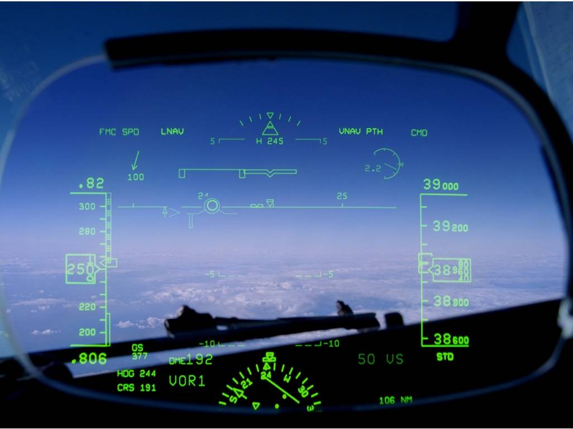
\includegraphics{hud}
  \caption{A Head-up Display \cite{hud_figure}}
\end{figure}

\noindent
Therefore, accurate data is critical in the field of aviation as pilots rely heavily on their instruments to ensure flight safety. Rockwell Collins values flight safety and strives to produce highly accurate data for all of their aviation systems. The current system uses the data from the aircraft\textquotesingle s precisely mounted and aligned IRU to update the HUD. However, the current system is unable to compensate for airframe droop that shifts the HUD from its precisely aligned position. Rockwell Collins sees a need for aviation HUD to be dynamically realigned during flight. Given the nature of avionic systems, a highly accurate solution is a must.\\\\
In fact, more accurate in flight data can be obtained by adding additional aircraft IRUs in separate physical locations within the aviation system. However, a drawback to this approach is the high cost of a single IRU installation. As a result, Rockwell Collins plans to explore the potential of mounting an inexpensive MEMS IRU onto the HUD itself. This additional IRU opens the possibility of comparing its output with the output of the aircraft\textquotesingle s precisely mounted and aligned IRU in order to quantify the HUDs alignment error. Our team hopes to develop an applicable solution to this real world problem afflicting flight safety.

\section*{Problem Solution}
Our goal is to develop a near real-time algorithm that will be able to determine the correct alignment dynamically during a flight environment by using data from both the inexpensive MEMS IRU and the aircraft mounted IRU. The algorithm will account for the HUD\textquotesingle s position and rotation to ensure that the conformal attitude, flight path information and other displayed data is accurately aligned. Accurate HUD alignment is achieved when the displayed information becomes a true representation of sensor data in relation to the HUD. Rockwell Collins desires a dynamic solution which utilizes inertial sensors to constantly measure and minimize the HUD alignment error with respect to the aircraft boresight.\\\\
To meet this desire, we will develop an algorithm that calculates the correct HUD alignment in real time using data from two separate sensors. Specifically, the algorithm will compare the outputs from a precise and pre-aligned aircraft IRU and an inexpensive MEMS IRU to quantify the alignment error. The goal is to adjust the data being displayed on the HUD to account for its shifting alignment during flight. In the case of airframe droop, the resulting alignment error might require the output data to be shifted vertically downwards while potentially rotating forward in order to compensate appropriately.\\\\
This algorithm will compensate for the airframe droop during flight to the desired accuracy level of one milliradian, which will result in a more dynamic alignment system. The end result of this project is to create a demonstration system to show a higher accuracy symbology output from the algorithm when coupled with two representative sensors (possibly simulated) and confirm against a known reference. In other words, we plan to show that the displayed data will be accurately represented even when the HUD shifts from its previous alignment. 

\section*{Problem Metrics}
Primarily, a functional program is fundamental for the entire project, this program should be able to recognize and read two groups of quaternion outputs from both inexpensive MEMS IRU and the aircraft\textquotesingle s IRUs. The program can be tested by looking at the data transmission behavior, the program is functional if it successfully receives the quaternion outputs from both IRUs in almost real time. Next, the algorithm of this program should be able to quantify and find the alignment error from the mounted IRUs. The outcome (aligned-data) of this algorithm should compensate the alignment error correctly, and the alignment error should be within a range of one milliradian. We may use unit tests for each part of the algorithm to check whether the data is processed correctly in each stage, and we may also transform the data into statistical data for deep analysis. In addition, the entire program is required to run in near real time. One complete cycle of the program consists of input of data, data processing output of data. The ideal algorithm should run in an accepted range of time and complexity for each cycle. 


\newpage
\nocite{*}
\bibliography{IEEEabrv, References}
\bibliographystyle{IEEEtran}


\newpage
	\section*{Signatures}
	\noindent\begin{tabular}{ll}
	\\[1cm]
	\makebox[2.5in]{\hrulefill} & \makebox[2.5in]{\hrulefill}\\
	Client & Date\\[8ex]% adds space between the two sets of signatures
	\makebox[2.5in]{\hrulefill} & \makebox[2.5in]{\hrulefill}\\
	Author 1 & Date\\[8ex]% adds space between the two sets of signatures
	\makebox[2.5in]{\hrulefill} & \makebox[2.5in]{\hrulefill}\\
	Author 2 & Date\\[8ex]% adds space between the two sets of signatures
	\makebox[2.5in]{\hrulefill} & \makebox[2.5in]{\hrulefill}\\
	Author 3 & Date\\[8ex]% adds space between the two sets of signatures
	\end{tabular}

\end{document}
